\chapter{拓扑流形}

%——————————————————————————————————%

本章开始把“状态空间”从一个集合提升为一个具有局部几何结构的空间。需要先区分两条相关但不同的主线：

\begin{itemize}
    \item \textbf{图册主线：}说明如何用局部欧氏坐标描述一个空间，以及如何在坐标图之间描述同一个点和同一条运动轨迹；
    \item \textbf{纤维丛主线：}说明每个空间点上还可以附着一类内部状态，并用投影、纤维和截面组织这些状态。
\end{itemize}

对于后续的可微流形、曲线、速度和切空间，图册主线是主要入口；纤维丛先作为预告，用来建立“切丛、余切丛和向量丛”的整体直觉。两条主线可以分别概括为
\[
\begin{aligned}
&\text{拓扑流形 }M
\longrightarrow \text{局部坐标图 }(U,x)
\longrightarrow x(U)\subset\R^d,\\
&\text{图的重叠}
\longrightarrow \text{坐标转换 }y\circ x^{-1}
\longrightarrow \text{可微兼容性},\\
&\text{轨迹 }\gamma:\R\to M
\longrightarrow \text{局部轨迹 }x\circ\gamma:\R\to\R^d
\longrightarrow \text{速度与切向量};
\end{aligned}
\]
\[
\begin{aligned}
&\text{总空间 }E\xrightarrow{\ \pi\ }\text{底空间 }M,\\
&p\in M\longrightarrow F_p=\pi^{-1}(\{p\})\subset E,\\
&\text{局部平凡化}
\longrightarrow \pi^{-1}(U)\cong U\times F
\longrightarrow \text{截面、丛态射与拉回丛}.
\end{aligned}
\]

前一条链回答“怎样在一个空间上做局部坐标微积分”，后一条链回答“每个空间点上附着的状态怎样随空间组织起来”。第四章将沿第一条链定义可微流形和切空间；第五章再把旋转与位姿的群结构加入其中。

%——————————————————————————————————%

\section{流形的基本语言}

\subsection{为什么需要局部欧氏空间}

在第一章和第二章中，我们把状态看作集合，把连续性看作拓扑性质。这样的语言可以描述哪些点彼此接近、轨迹是否连续，以及一个区域是否紧或连通，但还不能直接谈“速度”。

例如，粒子在球面上运动时，真实轨迹是
\[
    \gamma:\R\to S^2,\qquad t\mapsto\gamma(t).
\]
它的值是球面上的点，而不是任意的三维向量。我们可以把球面嵌入$\R^3$中画出来，但“球面上的点”和“该点在某张地图上的坐标”仍然是两个不同的对象。要计算速度，需要在每个点附近找到一个与欧氏空间开集同胚的局部区域。

\begin{definition}[拓扑流形]
设$M$是一个拓扑空间。若$M$满足以下条件，则称$M$为$n$维拓扑流形：
\begin{enumerate}
    \item $M$是Hausdorff空间；
    \item $M$是第二可数的；
    \item 对任意$p\in M$，存在包含$p$的开集$U\subset M$，以及$\R^n$中的开集$W$，使得$U$与$W$同胚。
\end{enumerate}
\end{definition}

第三个条件是流形定义的核心：每一个点附近都像$n$维欧氏空间。这里的“像”只表示拓扑同胚，不表示$M$整体就是$\R^n$。Hausdorff性保证不同点可以用不交邻域区分，第二可数性则排除了过大的病态空间，并保证许多局部构造可以用可数资料描述。

\begin{remark}[局部与整体]
直线$\R$是一维流形，圆周$S^1$也是一维流形。它们在每一个足够小的邻域中都像$\R$，但圆周整体上闭合，不能用一条实数坐标无奇点地覆盖。流形的关键正是：局部模型可以简单，整体结构不必简单。
\end{remark}

\subsection{坐标图}

\begin{definition}[坐标图]
设$M$是$n$维拓扑流形。一张坐标图（chart）是二元组$(U,x)$，其中$U\subset M$是开集，且
\[
    x:U\longrightarrow x(U)\subset\R^n
\]
是同胚，$x(U)$是$\R^n$中的开集。
\end{definition}

坐标图中有三个层次：
\[
    p\in U\subset M,\qquad
    x:U\to x(U),\qquad
    x(p)\in\R^n.
\]
其中$p$是流形上的真实点，$x$是坐标映射，$x(p)$只是这个点在当前坐标图下的表示。必须区分
\[
    p\neq x(p).
\]
这与地球表面上的真实地点和地图上的经纬度很相似：地图坐标可以改变，真实地点没有因此改变。

\begin{proposition}[局部欧氏表示]
若$(U,x)$是$n$维流形上的坐标图，则$U$中的每个点都可以由$n$个实数局部表示。流形上的局部问题因此可以转写为$\R^n$中的问题。
\end{proposition}

\subsection{图册}

\begin{definition}[图册]
一族坐标图
\[
    \mathcal A=\{(U_\alpha,x_\alpha)\}_{\alpha\in I}
\]
若满足
\[
    M=\bigcup_{\alpha\in I}U_\alpha,
\]
则称$\mathcal A$为$M$的一个图册（atlas）。
\end{definition}

图册只要求所有局部区域覆盖整个流形。它不要求一张图覆盖全部$M$，也不要求不同图使用相同的坐标公式。球面需要多张地图，正是图册思想的最直观例子。

\begin{definition}[坐标转换]
设$(U,x)$和$(V,y)$是两张坐标图，且$U\cap V\neq\varnothing$。在重叠区域内，从$x$坐标转换到$y$坐标的映射为
\[
    y\circ x^{-1}:
    x(U\cap V)\longrightarrow y(U\cap V).
\]
其逆映射为
\[
    x\circ y^{-1}:
    y(U\cap V)\longrightarrow x(U\cap V).
\]
\end{definition}

读坐标转换的顺序是：
\[
    x(p)
    \xrightarrow{\ x^{-1}\ }p
    \xrightarrow{\ y\ }y(p).
\]
因此对每个$p\in U\cap V$，
\[
    (y\circ x^{-1})(x(p))=y(p).
\]
坐标转换描述的是同一个流形点的两种坐标，而不是把一个物理点变成了另一个物理点。

\begin{center}
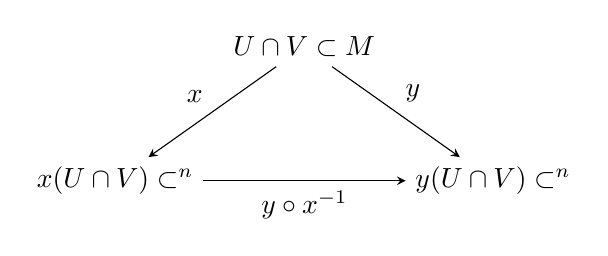
\begin{tikzpicture}[>=stealth]
    \node (M) at (0,1.7) {$U\cap V\subset M$};
    \node (X) at (-2.4,0) {$x(U\cap V)\subset\R^n$};
    \node (Y) at (2.4,0) {$y(U\cap V)\subset\R^n$};
    \draw[->] (M) -- node[above left] {$x$} (X);
    \draw[->] (M) -- node[above right] {$y$} (Y);
    \draw[->] (X) -- node[below] {$y\circ x^{-1}$} (Y);
\end{tikzpicture}
\end{center}

\subsection{连续兼容与可微兼容}

对于拓扑流形中的两张坐标图，$x$和$y$本身都是同胚，所以在重叠区域上$y\circ x^{-1}$自动是同胚。换句话说，拓扑流形中的坐标转换已经具有$C^0$层面的兼容性。

但同胚不保证可微。若希望在坐标图中对曲线求导，就必须进一步要求坐标转换具有足够的光滑性：
\[
    y\circ x^{-1}
    \quad\text{和}\quad
    x\circ y^{-1}
\]
都应为相应阶数的可微映射。把这类兼容的坐标图组成图册，就得到可微结构；把所有与之兼容的图收集起来，则得到极大可微图册。这个过程将在第四章正式定义。

\begin{remark}[为什么坐标兼容性重要]
在图$x$中得到的坐标速度，换到图$y$后要通过坐标转换的Jacobian变换。如果坐标转换不可微，两个坐标系统中的速度就不能通过统一的链式法则比较。因此，“图册覆盖空间”只解决了局部表示问题；“图册之间光滑兼容”才解决了微积分的一致性问题。
\end{remark}

%——————————————————————————————————%

\section{图册主线：从轨迹到局部运动}

\subsection{流形上的连续轨迹}

经典粒子的运动可以表示为一条从时间轴到状态空间的映射
\[
    \gamma:\R\longrightarrow M,\qquad
    t\longmapsto\gamma(t).
\]
其中$\gamma(t)$是时刻$t$的真实状态或位置。若粒子运动没有突然跳跃，则$\gamma$应为连续映射。

给定$p=\gamma(t_0)$，取一张包含$p$的坐标图$(U,x)$。轨迹在这张局部地图中的表示为
\[
    x\circ\gamma:
    \gamma^{-1}(U)\subset\R
    \longrightarrow x(U)\subset\R^n,
    \qquad
    t\longmapsto x(\gamma(t)).
\]
由于$\gamma$连续且$U$是开集，$\gamma^{-1}(U)$是时间轴中的开集，所以局部轨迹在$t_0$附近至少有一个开放的定义区间。

\begin{center}
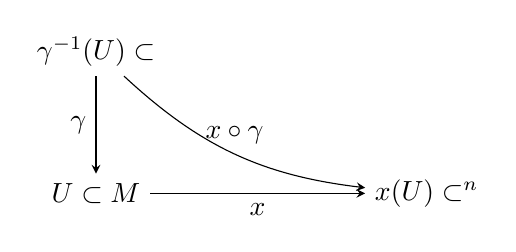
\begin{tikzpicture}[>=stealth]
    \node (T) at (0,1.8) {$\gamma^{-1}(U)\subset\R$};
    \node (M) at (0,0) {$U\subset M$};
    \node (E) at (4.2,0) {$x(U)\subset\R^n$};
    \draw[->] (T) -- node[left] {$\gamma$} (M);
    \draw[->] (M) -- node[below] {$x$} (E);
    \draw[->] (T) to[bend right=18] node[above] {$x\circ\gamma$} (E);
\end{tikzpicture}
\end{center}

这张图给出从真实运动到欧氏计算的基本链条：
\[
    t\longmapsto\gamma(t)\longmapsto x(\gamma(t)).
\]
在流形上，$\gamma(t)$和$x(\gamma(t))$不是同一个对象；前者属于$M$，后者属于$\R^n$。

\subsection{坐标速度的转换}

假设$(U,x)$和$(V,y)$在轨迹附近重叠，坐标转换光滑，且局部轨迹可微。对同一条轨迹有
\[
    y\circ\gamma
    =
    (y\circ x^{-1})\circ(x\circ\gamma).
\]
在$t_0$处对两边求导，形式上得到
\[
    \frac{\mathrm d}{\mathrm dt}y(\gamma(t))\bigg|_{t=t_0}
    =
    D(y\circ x^{-1})(x(p))
    \frac{\mathrm d}{\mathrm dt}x(\gamma(t))\bigg|_{t=t_0},
    \qquad p=\gamma(t_0).
\]
左边和右边是同一个瞬时运动在两套坐标中的分量表示。这个公式依赖坐标转换的可微性，而不是依赖某一张地图具有特殊地位。

\begin{remark}[连续与可微是两件事]
连续轨迹只说明$t$的微小变化会导致流形点的微小变化；它不保证速度存在。若轨迹的局部坐标表示可微，则称轨迹可微。可微结构保证“在一张图中可微”与“在另一张兼容图中可微”是等价的。
\end{remark}

\subsection{与SLAM状态估计的联系}

在SLAM中，状态空间可能是
\[
    \mathcal X
    =
    \SE(3)^N\times\R^{3K},
\]
也可能包含偏置、尺度、时间偏移或其他受约束变量。即使代码中使用矩阵、四元数或局部参数向量存储状态，真正的状态仍是流形上的点。

局部坐标的作用是把当前估计附近的状态变化表示成欧氏向量；它并不意味着整个状态空间就是一个全局欧氏空间。第四章将进一步说明：
\[
    \text{流形上的点}
    \quad\longleftrightarrow\quad
    \text{局部坐标中的增量},
\]
以及为什么增量应先在线性切空间中求解，再通过适当的流形更新返回状态空间。

%——————————————————————————————————%

\section{纤维丛预告：每个点附着内部状态}

\subsection{从底空间到总空间}

图册描述“底层空间本身如何被局部坐标覆盖”。纤维丛描述另一种结构：底空间中的每个点上方，还附着一个内部状态空间。

\begin{definition}[投影与纤维]
设$E$和$M$是拓扑空间，$\pi:E\to M$是连续满射。称$E$为总空间（total space），$M$为底空间（base space），$\pi$为投影（projection）。

对$p\in M$，定义$p$上方的纤维为
\[
    F_p:=\pi^{-1}(\{p\})
    =\{e\in E:\pi(e)=p\}.
\]
常把$\pi^{-1}(p)$作为$\pi^{-1}(\{p\})$的简写。
\end{definition}

投影$\pi$忘掉总空间元素中的附加状态，只保留它位于哪个底点。元素$e\in E$属于$p$上方的纤维，当且仅当$\pi(e)=p$。

\begin{center}
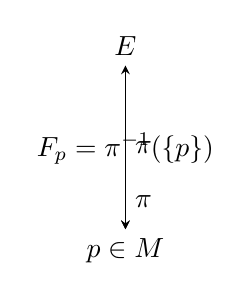
\begin{tikzpicture}[>=stealth]
    \node (E) at (0,2.1) {$E$};
    \node (F) at (0,0.8) {$F_p=\pi^{-1}(\{p\})$};
    \node (P) at (0,-0.5) {$p\in M$};
    \draw[->] (E) -- node[right] {$\pi$} (P);
    \draw[->] (F) -- (E);
    \draw[->] (F) -- node[right] {$\pi$} (P);
\end{tikzpicture}
\end{center}

物理上，可以把$M$理解为“物体在哪儿”，把$F_p$理解为“物体在$p$处还能取哪些内部状态”。例如，球面$S^2$上的每个点可以附着一个切平面；刚体的位置上可以附着姿态、速度或其他内部变量。但“位置加内部状态”是否是乘积，取决于具体配置空间的定义，不能仅凭物理语言自动断定。

\subsection{乘积丛与局部平凡化}

\begin{definition}[乘积丛]
给定拓扑空间$M$和$F$，令
\[
    E=M\times F,
    \qquad
    \pi:M\times F\longrightarrow M,
    \qquad
    \pi(p,f)=p.
\]
对任意$p\in M$，
\[
    F_p=\pi^{-1}(\{p\})=\{p\}\times F\cong F.
\]
这个丛称为乘积丛或平凡丛。
\end{definition}

直观地说，$M\times F$是在底空间的每个点上挂一份完全相同的$F$。例如
\[
    E=\R\times\R^2
\]
可以理解为：沿一条实轴的每个位置$x$，附着一个二维内部状态平面$\{x\}\times\R^2$。

\begin{definition}[纤维丛]
设$\pi:E\to M$是连续满射，$F$是一个拓扑空间。若对每个$p\in M$，存在包含$p$的开邻域$U\subset M$以及同胚
\[
    \Phi_U:\pi^{-1}(U)\longrightarrow U\times F,
\]
使得
\[
    \operatorname{pr}_1\circ\Phi_U=\pi,
    \qquad
    \operatorname{pr}_1:U\times F\to U,
\]
则称$\pi:E\to M$为以$F$为典型纤维的纤维丛。
\end{definition}

条件$\operatorname{pr}_1\circ\Phi_U=\pi$说明$\Phi_U$不仅是总空间之间的同胚，还必须保持底点不变。也就是说，对每个$e\in\pi^{-1}(U)$，
\[
    \Phi_U(e)=(\pi(e),f)
\]
的第一个分量必须是$e$原来投影到的底点。

若在光滑范畴中讨论纤维丛，则上述同胚和局部平凡化都应替换为相应的微分同胚和光滑映射。

\begin{center}
\begin{tikzpicture}[>=stealth]
    \node (EU) at (0,1.8) {$\pi^{-1}(U)$};
    \node (U) at (0,-0.1) {$U$};
    \node (PU) at (4.2,1.8) {$U\times F$};
    \node (U2) at (4.2,-0.1) {$U$};
    \draw[->] (EU) -- node[left] {$\pi$} (U);
    \draw[->] (PU) -- node[right] {$\operatorname{pr}_1$} (U2);
    \draw[->] (EU) -- node[above] {$\Phi_U$} (PU);
    \draw[->] (U) -- node[below] {$\mathrm{id}_U$} (U2);
\end{tikzpicture}
\end{center}

这就是局部平凡性（local triviality）：每一个足够小的底空间区域上方，纤维丛都看起来像普通乘积$U\times F$。真正可能复杂的是不同区域之间如何拼接。

\begin{remark}[平凡与局部平凡]
若整个丛存在与投影相容的丛同构
\[
    E\cong M\times F,
\]
则称其为平凡丛。纤维丛的定义本身要求局部平凡，但局部平凡不推出全局平凡。局部坐标简单、整体结构复杂，是图册和纤维丛共同体现的局部—整体思想。
\end{remark}

\subsection{圆柱与莫比乌斯带}

令底空间为$S^1$，典型纤维为区间$I=[-1,1]$。

圆柱可以写成
\[
    S^1\times[-1,1]\xrightarrow{\ \operatorname{pr}_1\ }S^1.
\]
它的每根纤维为$\{\theta\}\times[-1,1]$，总空间就是乘积，因此是平凡丛。

莫比乌斯带也有投影
\[
    \pi:\mathrm{Mobius}\longrightarrow S^1,
\]
每根纤维仍然同胚于$[-1,1]$。在$S^1$的任意足够小的弧段$U$上，它都可以展开为
\[
    \pi^{-1}(U)\cong U\times[-1,1].
\]
然而沿底圆绕行一周后，纤维发生一次翻转，因而不能在全局上写成$S^1\times[-1,1]$。

\begin{proposition}[莫比乌斯带的局部—整体性质]
莫比乌斯带是局部平凡但全局非平凡的区间纤维丛。它不是“非局部平凡的纤维丛”。
\end{proposition}

这里的区别很重要：如果一个对象连局部平凡性都不满足，通常就不应称为本章意义下的纤维丛；非平凡只表示它不能被一个全局乘积坐标系展开。

\subsection{截面：连续地选择每根纤维中的一个元素}

\begin{definition}[截面]
纤维丛$\pi:E\to M$的一个连续截面（section）是连续映射
\[
    \sigma:M\longrightarrow E
\]
满足
\[
    \pi\circ\sigma=\mathrm{id}_M.
\]
\end{definition}

逐点写出截面条件：
\[
    p\in M
    \xrightarrow{\ \sigma\ }\sigma(p)\in E
    \xrightarrow{\ \pi\ }p\in M.
\]
所以$\sigma(p)$一定属于$F_p$。截面不是总空间中的任意曲线，而是对底空间中的每个点恰好选择一个位于其上方纤维中的元素，并且这种选择随$p$连续（在相应范畴中还应光滑）。

在局部平凡化$\Phi_U$下，截面限制到$U$后满足
\[
    \Phi_U(\sigma(p))=(p,s_U(p)),
    \qquad
    s_U:U\to F.
\]
因此，局部平凡化中的截面确实由一个普通函数$s_U$表示。但不同平凡化下的函数必须通过过渡函数相容地拼接；全局上不一定存在单一函数$M\to F$表示截面。

\subsection{切丛预告：向量场是截面}

在第四章定义切空间之后，对每个$p\in M$都有一个切空间$T_pM$。把所有切空间不交并在一起，得到切丛
\[
    TM=\bigsqcup_{p\in M}T_pM,
    \qquad
    \pi:TM\to M,
    \qquad
    \pi(p,v)=p.
\]
其纤维为
\[
    \pi^{-1}(\{p\})=T_pM.
\]

对球面而言，$S^2$上的每个点附着一个切平面：
\[
    TS^2=\bigsqcup_{p\in S^2}T_pS^2.
\]
一个向量场是一个截面
\[
    X:S^2\to TS^2,
    \qquad
    \pi\circ X=\mathrm{id}_{S^2},
\]
也就是在每个$p$处选择一个切向量$X_p\in T_pS^2$。

这比把向量场简单写成函数$X:M\to\R^n$更本质，因为不同点的切向量属于不同的切空间：
\[
    T_pM\neq T_qM
\]
通常不能把它们当作同一个固定向量空间中的向量直接相加或比较。局部坐标可以给出分量表示，但不能抹掉切向量所属的基点。

\begin{remark}[为什么纤维丛先作为预告]
切丛、余切丛、向量丛和主丛都建立在“每个底点上附着一根纤维”的思想上。本章只需要掌握投影、局部平凡化和截面的结构；切空间上的线性运算、向量场和微分形式将在第四章展开。
\end{remark}

\subsection{限制丛、丛态射与丛同构}

\begin{definition}[限制丛]
设$\pi:E\to M$是纤维丛，$N\subset M$是子空间或子流形。将底空间限制到$N$，定义
\[
    E\vert_N
    :=
    \pi^{-1}(N)
    =
    \{e\in E:\pi(e)\in N\},
\]
并配备投影
\[
    \pi\vert_N:E\vert_N\to N,
    \qquad
    e\longmapsto\pi(e).
\]
所得丛称为$\pi$在$N$上的限制丛。
\end{definition}

限制丛只保留$N$上方的纤维。例如，若$E$定义在整个球面上，而只研究北半球$N\subset S^2$，就可以把$E$限制到$N$。严格的子丛还需要要求每根纤维是原纤维中具有适当结构的子空间；“限制丛”只是按底空间取逆像。

\begin{definition}[丛态射]
给定两个纤维丛
\[
    \pi:E\to M,
    \qquad
    \pi':E'\to M',
\]
一对连续映射
\[
    u:E\to E',
    \qquad
    f:M\to M'
\]
若满足
\[
    \pi'\circ u=f\circ\pi,
\]
则称$(u,f)$为丛态射。
\end{definition}

逐点写出交换条件：
\[
    e\in F_p=\pi^{-1}(\{p\})
    \quad\Longrightarrow\quad
    u(e)\in F'_{f(p)}.
\]
也就是说，丛态射不仅要搬运总空间元素，还要尊重元素所属的纤维。

\begin{center}
\begin{tikzpicture}[>=stealth]
    \node (E) at (0,1.8) {$E$};
    \node (M) at (0,-0.1) {$M$};
    \node (Ep) at (4.2,1.8) {$E'$};
    \node (Mp) at (4.2,-0.1) {$M'$};
    \draw[->] (E) -- node[left] {$\pi$} (M);
    \draw[->] (Ep) -- node[right] {$\pi'$} (Mp);
    \draw[->] (E) -- node[above] {$u$} (Ep);
    \draw[->] (M) -- node[below] {$f$} (Mp);
\end{tikzpicture}
\end{center}

若$(u,f)$存在反向丛态射$(u^{-1},f^{-1})$，则称其为丛同构。若$M=M'$且$f=\mathrm{id}_M$，则是在同一个底空间上比较两个纤维丛结构。

\subsection{拉回丛}

拉回丛把一个已经定义在旧底空间上的纤维结构，沿着连续的底空间映射带回新的底空间。设
\[
    \pi:E\to M,
    \qquad
    f:M'\to M.
\]
对$p'\in M'$，新丛在$p'$上方的纤维应当复制旧丛在$f(p')$上方的纤维：
\[
    (f^*E)_{p'}\cong E_{f(p')}.
\]

\begin{definition}[拉回丛]
定义
\[
    f^*E
    :=
    \{(p',e)\in M'\times E:
      f(p')=\pi(e)\}.
\]
投影定义为
\[
    \pi':f^*E\to M',
    \qquad
    \pi'(p',e)=p'.
\]
\end{definition}

约束$f(p')=\pi(e)$保证$e$确实位于旧丛中$f(p')$上方的纤维。自然的总空间映射为
\[
    \widehat f:f^*E\to E,
    \qquad
    \widehat f(p',e)=e.
\]
于是
\[
    \pi\bigl(\widehat f(p',e)\bigr)
    =
    \pi(e)
    =
    f(p')
    =
    f\bigl(\pi'(p',e)\bigr),
\]
即
\[
    \pi\circ\widehat f=f\circ\pi'.
\]

\begin{center}
\begin{tikzpicture}[>=stealth]
    \node (PB) at (0,1.8) {$f^*E$};
    \node (MP) at (0,-0.1) {$M'$};
    \node (E) at (4.2,1.8) {$E$};
    \node (M) at (4.2,-0.1) {$M$};
    \draw[->] (PB) -- node[left] {$\pi'$} (MP);
    \draw[->] (E) -- node[right] {$\pi$} (M);
    \draw[->] (PB) -- node[above] {$\widehat f$} (E);
    \draw[->] (MP) -- node[below] {$f$} (M);
\end{tikzpicture}
\end{center}

拉回丛与协向量的拉回共享同一个几何思想：底空间映射$f$指向旧空间，而结构沿相反方向被带回。二者不是同一个构造：协向量拉回是线性映射的对偶操作，拉回丛则是通过纤维和交换图构造新的几何对象。

%——————————————————————————————————%

\section{常见的状态流形}

\subsection{圆与球面}

\begin{definition}[单位圆与单位球面]
单位圆和单位球面分别定义为
\[
    S^1=\{x\in\R^2:\|x\|=1\},
    \qquad
    S^2=\{x\in\R^3:\|x\|=1\}.
\]
更一般地，
\[
    S^n=\{x\in\R^{n+1}:\|x\|=1\}.
\]
\end{definition}

\begin{theorem}[球面为流形]
$S^n$是$n$维拓扑流形。
\end{theorem}

球面不能由一个全局欧氏坐标图无奇点地覆盖，但可以用多张局部图覆盖。例如，去掉球面的北极和南极后，可以分别使用立体投影得到两张坐标图。两张图在重叠区域的坐标转换，正是图册描述整体球面的方式。

\subsection{旋转空间}

\begin{definition}[特殊正交群]
三维旋转空间定义为
\[
    \SO(3)
    =
    \{R\in\R^{3\times3}:R^\top R=I,\ \det R=1\}.
\]
\end{definition}

这里先把$\SO(3)$看作一个拓扑流形。矩阵乘法和求逆赋予它的群结构将在第五章讨论。正交约束和行列式约束说明旋转矩阵不是$\R^9$中的任意点，而是一个低维的受限空间。

\begin{theorem}[$\SO(3)$的维数]
$\SO(3)$是三维拓扑流形，因此三维旋转在局部具有三个自由度。
\end{theorem}

\subsection{位姿空间}

\begin{definition}[特殊欧氏群]
三维刚体位姿空间定义为
\[
    \SE(3)
    =
    \left\{
    \begin{bmatrix}
        R&t\\
        0&1
    \end{bmatrix}
    :
    R\in\SO(3),\ t\in\R^3
    \right\}.
\]
\end{definition}

一个位姿同时包含旋转$R$和平移$t$。作为拓扑空间，它与$\SO(3)\times\R^3$同胚，因此
\[
    \dim\SE(3)=3+3=6.
\]

\begin{theorem}[$\SE(3)$的维数]
$\SE(3)$是六维拓扑流形。三维刚体位姿具有三个旋转自由度和三个平移自由度。
\end{theorem}

\begin{remark}[状态表示不是状态空间本身]
旋转矩阵有九个矩阵元素但只有三个局部自由度；四元数有四个分量但受到单位范数约束；局部旋转向量只有三个分量，但通常只能作为局部坐标。代码中的参数化是表示方式，不能直接替代状态空间的拓扑和几何结构。
\end{remark}

%——————————————————————————————————%

\section{商空间与规范自由度}

\subsection{商空间}

\begin{definition}[等价关系与商空间]
设$X$为拓扑空间，$\sim$为$X$上的等价关系。等价类集合记为
\[
    X/{\sim}
    =
    \{[x]:x\in X\},
    \qquad
    [x]=\{y\in X:y\sim x\}.
\]
这个集合配备商拓扑后称为商空间。
\end{definition}

自然投影为
\[
    q:X\to X/{\sim},
    \qquad
    q(x)=[x].
\]
商拓扑的定义是：集合$A\subset X/{\sim}$是开集，当且仅当$q^{-1}(A)$在$X$中是开集。商空间中的一个点不是$X$中的单个元素，而是一个等价类。

\begin{remark}[商空间与局部坐标]
商空间把“物理上不可区分”的多个表示合并为一个点。它可能仍然是一个良好的流形，也可能出现奇点或其他病态结构；不能仅凭等价关系就断定商空间一定是流形。
\end{remark}

\subsection{SLAM中的规范自由度}

设群$G$作用在状态空间$\mathcal X$上。若观测残差对该作用不变，即
\[
    r(g\cdot x)=r(x),
    \qquad
    \forall g\in G,\ x\in\mathcal X,
\]
则观测实际上不能区分同一轨道中的状态。此时，真正被观测的对象更接近商空间$\mathcal X/G$。

\begin{theorem}[残差下降到商空间]
若$r:\mathcal X\to\mathcal Z$满足
\[
    r(g\cdot x)=r(x),
\]
则存在映射$\bar r:\mathcal X/G\to\mathcal Z$，使得
\[
    r=\bar r\circ q,
\]
其中$q:\mathcal X\to\mathcal X/G$是自然投影。
\end{theorem}

\begin{corollary}[固定首帧]
在只依赖相对位姿的SLAM问题中，固定第一帧位姿是在每个规范等价类中选择一个代表元。它消除了表示层面的自由度，但不等于增加了新的物理观测。
\end{corollary}

规范处理与坐标图有相似之处：二者都在区分“真实几何对象”和“描述它的表示”。但坐标变换通常是在同一个流形点上切换局部坐标，规范商则可能把多个状态表示直接视为同一个物理状态。

%——————————————————————————————————%

\section{带边界流形与约束}

\subsection{带边界流形}

\begin{definition}[闭上半空间]
$n$维闭上半空间定义为
\[
    \mathbb H^n
    =
    \{(x^1,\ldots,x^n)\in\R^n:x^n\ge 0\}.
\]
\end{definition}

\begin{definition}[带边界流形]
若一个拓扑空间的每个点都有邻域同胚于$\mathbb H^n$中的相对开集，则称其为$n$维带边界流形。
\end{definition}

在局部坐标$x=(x^1,\ldots,x^n)$下，满足$x^n>0$的点是内部点，满足$x^n=0$的点是边界点。由所有边界点组成的集合记为$\partial M$。

\begin{remark}[边界是局部性质]
一个点是否在边界上，不取决于某张地图的画法，而取决于它在局部模型$\mathbb H^n$中是否对应到超平面$x^n=0$。换用另一张合法的边界坐标图后，这一性质保持不变。
\end{remark}

\subsection{约束状态空间}

满足不等式约束
\[
    g(x)\ge 0
\]
的可行集合，可能形成带边界或带角的空间。机器人运动范围、传感器视场、地图边界和物理接触约束都可能使状态空间不再是无边界的欧氏开集。

\begin{proposition}[边界对优化的影响]
拓扑上的边界意味着某些方向离开可行状态空间。因而在边界附近，简单的无约束欧氏增量模型可能不再合适，需要使用受约束更新、局部可行锥或其他与约束相容的优化模型。
\end{proposition}

这里暂不展开带角流形和边界上的微分结构；本章只保留一个判断原则：状态满足的约束不仅改变数值范围，也可能改变状态空间的局部拓扑模型。

%——————————————————————————————————%

\section{本章小结：对象、映射与局部—整体}

本章最重要的内容可以压缩为以下几条：

\begin{enumerate}
    \item 拓扑流形是一个满足Hausdorff性、第二可数性和局部欧氏性的拓扑空间。
    \item 一张图是
    \[
        x:U\to x(U)\subset\R^d,
    \]
    它把流形上的局部区域翻译成欧氏坐标；真实点$p$与坐标表示$x(p)$必须区分。
    \item 图册是一族覆盖$M$的坐标图；两张重叠图之间通过
    \[
        y\circ x^{-1}
    \]
    描述同一个点的坐标转换。
    \item 轨迹是映射
    \[
        \gamma:\R\to M,
    \]
    在局部图中变成
    \[
        x\circ\gamma:\gamma^{-1}(U)\to\R^d.
    \]
    坐标转换的光滑兼容性保证局部速度可以被解释为同一个抽象切向量。
    \item 一个纤维丛由投影
    \[
        \pi:E\to M
    \]
    组织；$E$是总空间，$M$是底空间，$p$上方的纤维是
    \[
        F_p=\pi^{-1}(\{p\}).
    \]
    \item 纤维丛不只要求每根纤维像同一个$F$，还要求局部平凡：
    \[
        \pi^{-1}(U)\cong U\times F.
    \]
    截面是满足$\pi\circ\sigma=\mathrm{id}_M$的映射；切丛的截面就是向量场。
    \item 商空间处理等价表示，带边界流形处理局部可行域；二者都说明状态空间的整体结构不能只由一组全局欧氏坐标代替。
\end{enumerate}

因此，后续几何主线可以写成
\[
    \text{轨迹}
    \longrightarrow
    \text{切向量}
    \longrightarrow
    \text{切丛}
    \longrightarrow
    \text{向量场}
    \longrightarrow
    \text{李群与李代数}
    \longrightarrow
    \text{位姿优化}.
\]
第四章从图册的可微兼容性开始，定义可微映射、切空间、向量场、推前、拉回和度量；第五章则把$\SO(3)$与$\SE(3)$的群结构加入这条链，解释为什么SLAM可以在切空间中求解增量，再在流形上进行合法更新。
